\chapter{Correlação Cruzada de Ruído Ambiental Sísmico}

\section{Introdução}

Os métodos para determinar a estrutura sísmica da Terra, em particular os métodos tomográficos, baseiam-se num princípio simples: a determinação das velocidades de propagação das ondas sísmicas e a procura de um modelo que melhor se ajuste às velocidades encontradas. A resolução dos modelos obtidos depende do tipo de onda utilizado e da geometria espacial das estações sismográficas segundo à fonte do sinal. \cite{aki_space_1957} propôs a utilização do ruído sísmico ambiental para medir a dispersão das ondas Rayleigh e Love nas camadas mais superficiais. Somente \cite{campillo_long-range_2003}  e \cite{shapiro_emergence_2004} mostraram, pela primeira vez, a  presença de ondas superficiais nas correlações cruzadas entre pares de estações.

\cite{campillo_long-range_2003}, \cite{shapiro_emergence_2004} e, principalmente, \cite{wapenaar_retrieving_2004} mostram que pode-se recuperar a resposta elástica da Terra a partir da correlação cruzada entre dois pontos em  um campo de ondas difuso ou aleatório. Essa resposta é aproximada como a Função de Green, como é mostrada na equação \ref{crosscorrelation}. 

\cite{boschi_measuring_2013} define a correlação cruzada ($C_{xy}(t,\omega)$) como: 
\begin{eqnarray}
\label{crosscorrelation}
C_{xy}(t,\omega) = \frac{1}{2\pi}\int_{-T}^{T}u_{1}(x,t,\omega)u_{2}(y,t+\tau,\omega) d\tau
\end{eqnarray}

onde $u_{1}$ e $u_{2}$ são sinais registrados em duas estações nas posições $x$ e $y$, $t$ é o tempo, $\omega$ é a frequência, $\tau$ é o atraso e o parâmetro $T$ define o tamanho da janela em que a correlação cruzada é computada.
\\

Por possuir inúmeras vantagens em relação aos métodos de análise tradicionais que utilizam dados de sismos para a tomografia sísmica, o número de artigos sobre a correlação de ruído ambiental cresceu bastante. \cite{shapiro_emergence_2004} lista as seguintes vantagens: as medidas podem ser realizadas em qualquer direção de propagação e não estão limitadas à geometria fonte-receptor; não dependem da localização da fonte; a zona de sensibilidade destas medições situa-se na região entre as duas estações; pode-se analisar pequenos períodos se existirem estações relativamente próximas umas das outras.

\cite{shapiro_emergence_2004} testaram se as funções de Green podem ser extraídas do ruído sísmico ambiental, neste teste eles selecionaram um
período relativamente calmo no nível de atividade sísmica mundial, onde não ocorreram sismos com magnitude maior que 7, com esses registos contínuos da componente vertical das estações ANMO e CCM nos Estados Unidos, podem ser observadas na Figura \ref{shapiro}-a), calcularam a correlação cruzada para diferentes bandas de período, mostrado na Figura \ref{shapiro}-b), e aplicaram a análise tempo/frequência,desenvolvida por \cite{levshin_automated_2001}, para calcular a velocidade de grupo das ondas de superfície. \cite{shapiro_emergence_2004} compararam as características de dispersão do sinal emergente com resultados obtidos de métodos que utilizam dados de sismos para o mesmo trajeto.  Nesta comparação verificaram que os resultados obtidos para os dois casos são semelhantes.

\begin{figure}[!ht]
\centering
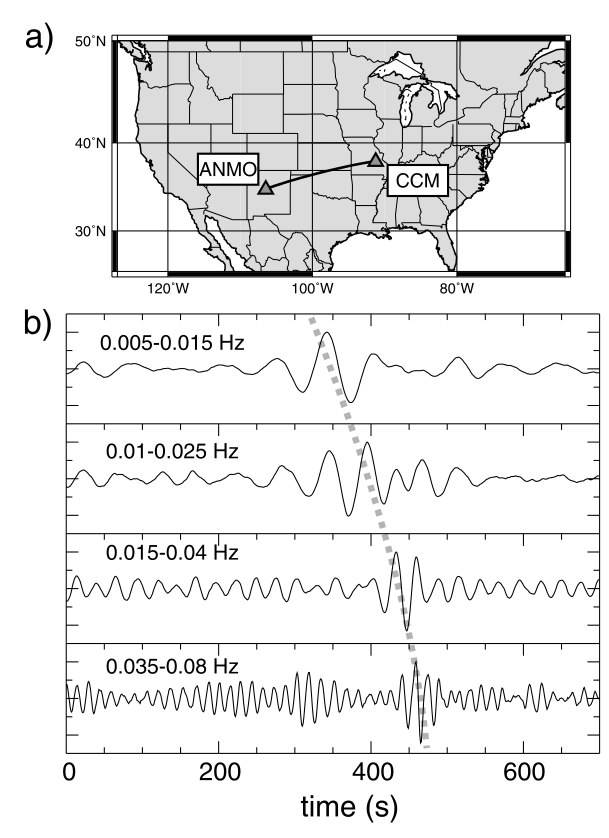
\includegraphics[scale=0.5]{Figs/shapiro2004.png}
\caption{a) Mapa mostrando a localização das estações. b) Correlações cruzadas da componente vertical dos registros com diferentes filtros de passa-banda, indicados na parte esquerda superior. Linha pontilhada dá ênfase na dispersão do sinal emergente. Extraído de \cite{shapiro_emergence_2004}.}
\label{shapiro}
\end{figure} 

\section{Processamento}

Para o processamento dos dados utilizou-se o código escrito pelo Professor Bruno Goutorbe do departamento de Geologia da Universidade Federal Fluminense. Tal código engloba: preparação dos dados, cálculo da correlação, análise Tempo/frequência e inversão tomográfica.  O código está disponível no repositório do GitHub: https://github.com/bgoutorbe/seismic-noise-tomography.

Conceitualmente o fluxo de preparação e processamento é baseado no trabalho de \cite{bensen_processing_2007}, porém algumas alterações na filtragem espectral  foram feitas devido a utilização de dados de média a alta frequência. O fluxograma \ref{fluxograma_bensen2007} representa um resumo do processamento, cada etapa mostrada no fluxograma terá uma explicação sintetizada nos tópicos a seguir.

\begin{figure}[!ht]
\centering
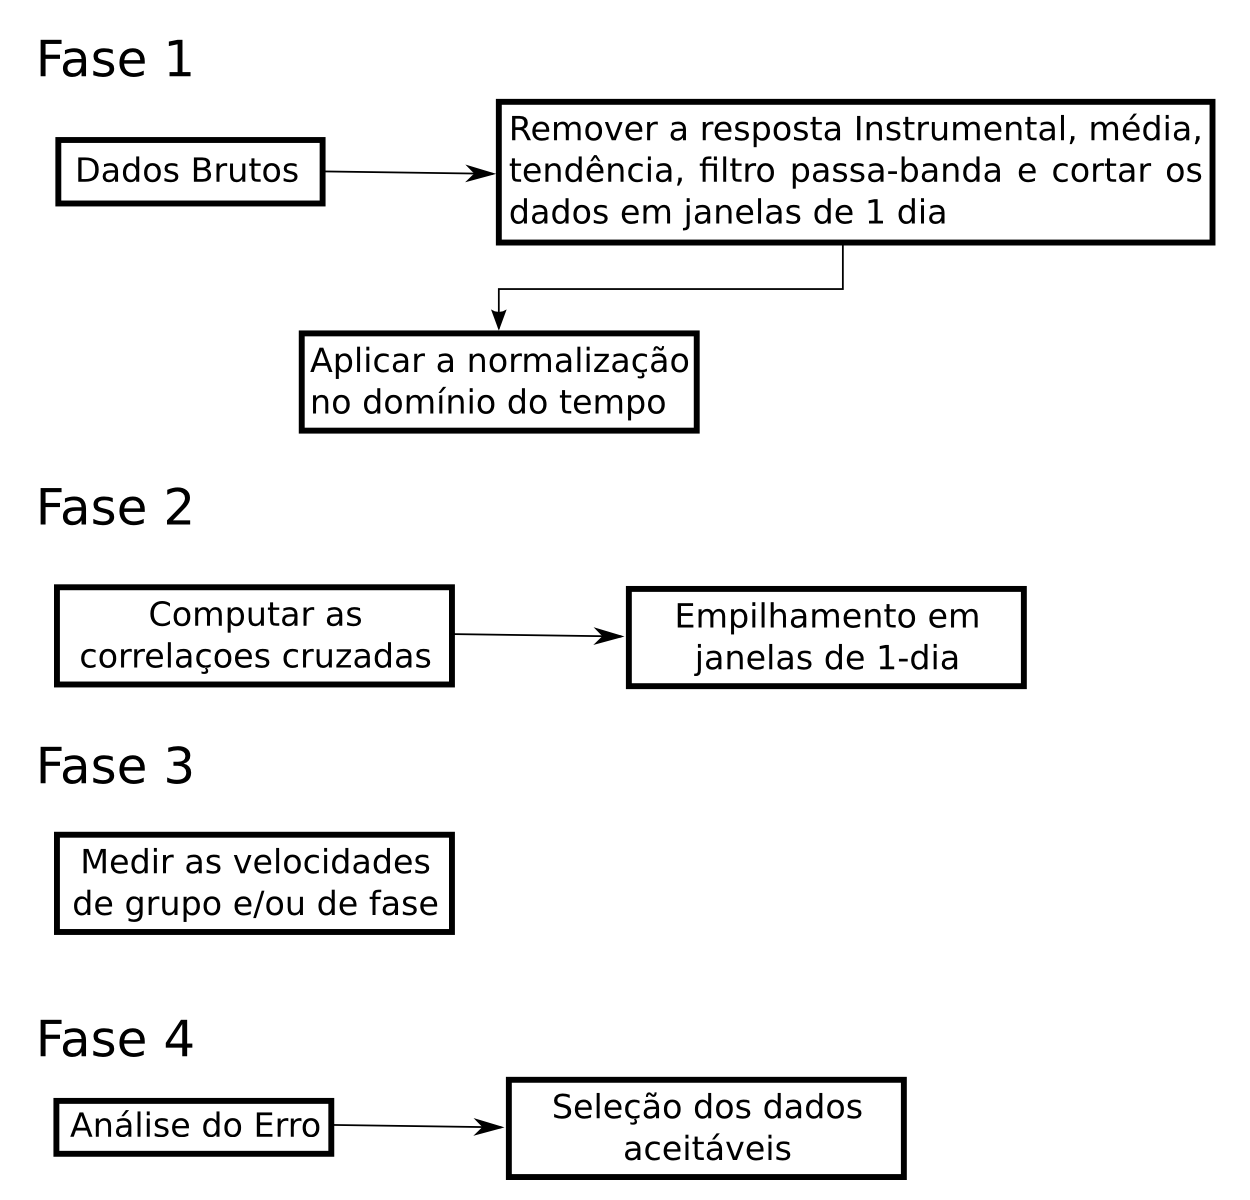
\includegraphics[scale=0.5]{Figs/fluxograma_bensen2007.png}
\caption[Representação esquemática do processamento.]{Representação esquemática do processamento. Fase 1 - etapas que involvem a preparação dos dados antes da correlação. Fase 2 - esboços do processo de correlação cruzada e empilhamento. Fase 3 -Medidas de dispersão. Fase 4 - Análise do Erro e seleção de dados aceitáveis. Adaptado de \cite{bensen_processing_2007}.}
\label{fluxograma_bensen2007}
\end{figure} 

\subsection{Preparação dos dados para cada estações}

\cite{bensen_processing_2007} cita que a primeira fase do processamento  é feita para preparar os dados da forma da onda de cada estação individualmente. Faz-se isso para acentuar o ruído ambiental de banda larga e para remover os sinais de terremoto e de irregularidades instrumentais que tendem a ocultar o ruído ambiental.

Segundo \cite{bensen_processing_2007}, séries temporáis diárias com menos que 80\% do registro devem ser rejeitadas, mas isso varia de acordo com a discretização do usuário. No caso desse trabalho foram utilizados séries  temporáis diárias com 99\% do registro, com o propósito de usar o mínimo possível a interpolação para preencher as lacunas nos registros.

\cite{bensen_processing_2007} mostra que um passo importante na preparação dos dados é a "normalização temporal" ou "normalização no domínio do tempo". Isto é feito para reduzir na correlação cruzada os efeitos de terremotos, irregularidades instrumentais e fontes de ruídos não-estacionários próximos á estação. \cite{bensen_processing_2007} compara cinco métodos diferentes para a normalização temporal, como observado na Figura \ref{temporal_norma}.

\begin{figure}[!ht]
\centering
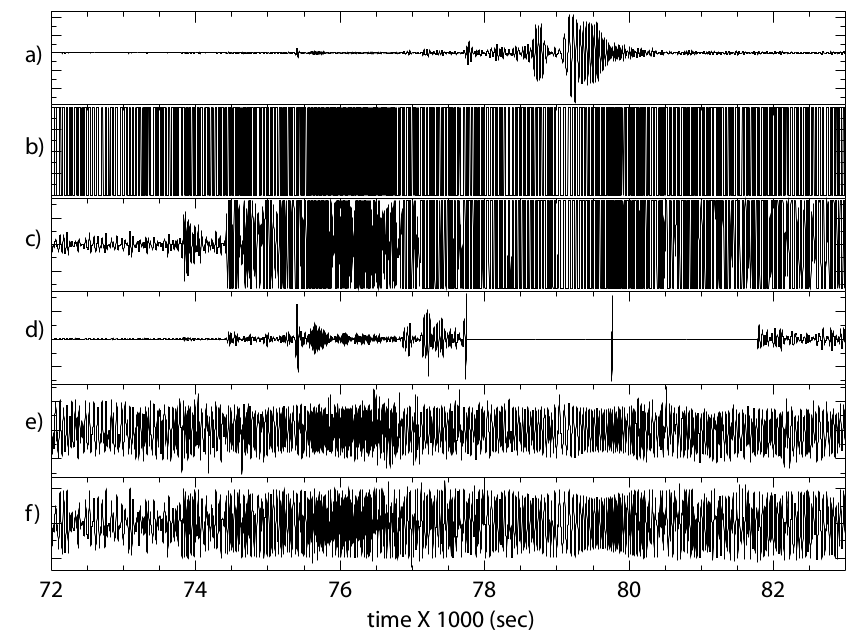
\includegraphics[scale=0.4]{Figs/temporal_norma.png}
\caption[Formas de onda mostrando exemplos de cinco tipos de normalização no dominio do tempo.]{Formas de onda mostrando exemplos de cinco tipos de normalização no dominio do tempo testadas por \cite{bensen_processing_2007}. Os exemplos estão com o filtro passa-banda entre 20 e 100 segundos e mostram a contaminação por sinais de terremoto. (a)  Dado bruto mostrando 3 horas de dados janelados em torno de um grande terremoto (M = 7.2, Afeganistão) registrado na estação ANMO. (b) Normalização 1-bit. (c) Forma de onda cortada, onde o limiar de recorte é igual ao rms da amplitude do sinal de um dado dia. (d) Evento detectado e removido automaticamente. (e) Normalização da média absoluta móvel. (f) Normalização ‘\textit{water level}’. Retirado de \cite{bensen_processing_2007}.}
\label{temporal_norma}
\end{figure} 

Terremotos geram grandes impecílios na automatização do processamento, pois eles ocorrem irregularmente e apenas grandes terremotos são encontrados nos catálogos globais, como visto na na Figura \ref{temporal_norma}-a. Então a remoção dos sinais dos terremotos tem que ser adaptativa aos dados. Muitos estudos aplicam a técnica da "normalização 1-bit", como observado na Figura \ref{temporal_norma}-b, em que somente o sinal da série temporal é retido (+1 ou -1) e a amplitude é completamente ignorada. Neste trabalho foi aplicado a "normalização da média absoluta móvel", esta produz uma razão sinal-ruído maior que a normalização 1-bit no conjunto de dados. Como mostra \cite{seats_improved_2012} em seus estudos. A "normalização da média absoluta móvel" é calculada na janela de terremotos (15 a 50 segundos) para isolar os terremotos que não são visíveis no sinal bruto.

\subsection{Normalização espectral ou braqueamento}

O Ruído Sísmico Ambiental não é branco no domínio da frequência, ou seja, tem frequências que se destacam. \cite{bensen_processing_2007} cita que a normalização espectral atua para alargar a banda do sinal nas correlações cruzadas e atua contra a degradação causada por fontes persistentes, como mostrado na Figura \ref{whitening}. Portanto, fez-se uso da normalização espectral nos dados brutos para tentar diminuir a esse efeito.

\begin{figure}[!ht]
\centering
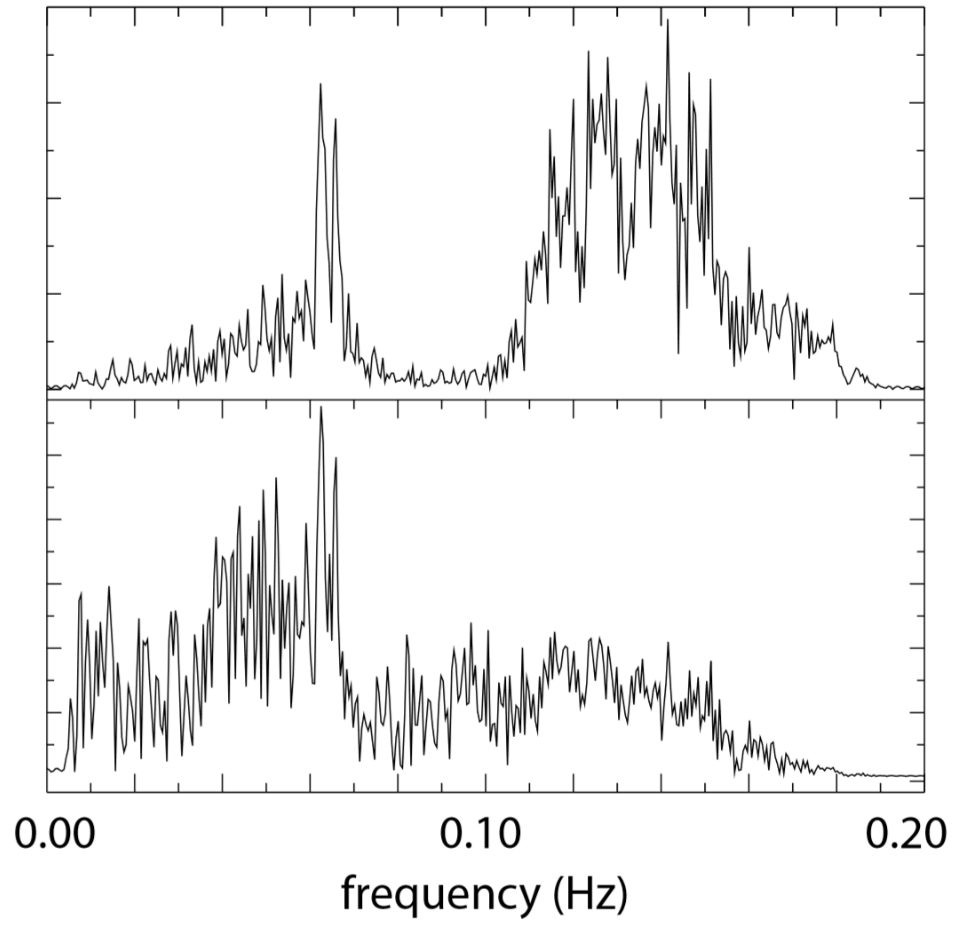
\includegraphics[scale=0.5]{Figs/whitening.png}
\caption[Comparação entre correlações com e sem  normalização espectral.]{Comparação entre correlações com e sem  normalização espectral. Correlação cruzada das estações CCM e SSPA (Standing Stone, PA, USA) filtrada entre 7 e 150 segundos.}
\label{whitening}
\end{figure} 

A janela temporal  utilizada por \cite{bensen_processing_2007} em seu trabalho é de 7 a 150 segundos, porém quando a distância entre as estações é pequena ($\simeq 20 km$) é necessário utilizar períodos mais curtos, como é o caso desse trabalho. A banda de interesse desta dissertação é de 2 a 50 segundos, logo inclui-se o ruído de alta frequência no processamento. Com a necessidade de preservar este ruído de alta frequência, não se aplicou a normalização espectral nas correlações cruzadas calculadas. Testes preliminares com a normalização espectral nas correlações cruzadas calculadas mostraram que com a normalização espectral dos dados a qualidade em curtos períodos era menor. 


\subsection{Correlação Cruzada, Empilhamento e  Sinal emergente}

Após preparar as séries temporais diárias, a próxima fase, como visto na Figura \ref{fluxograma_bensen2007}, é computar as correlações cruzadas e o empilhamento, mostrados na Figura \ref{correlacao_cruzada}. \cite{bensen_processing_2007} mostra que mesmo com distâncias entre as estações sendo muito longas ou curtas deve-se fazer a correlação entre todas os pares de estações possíveis. No futuro deve-se fazer a seleção das medidas aceitáveis. O número total de pares de estações possíveis é dado por $n(n-1)/2$, onde $n$ é o número de estações.

\begin{figure}[!ht]
\centering
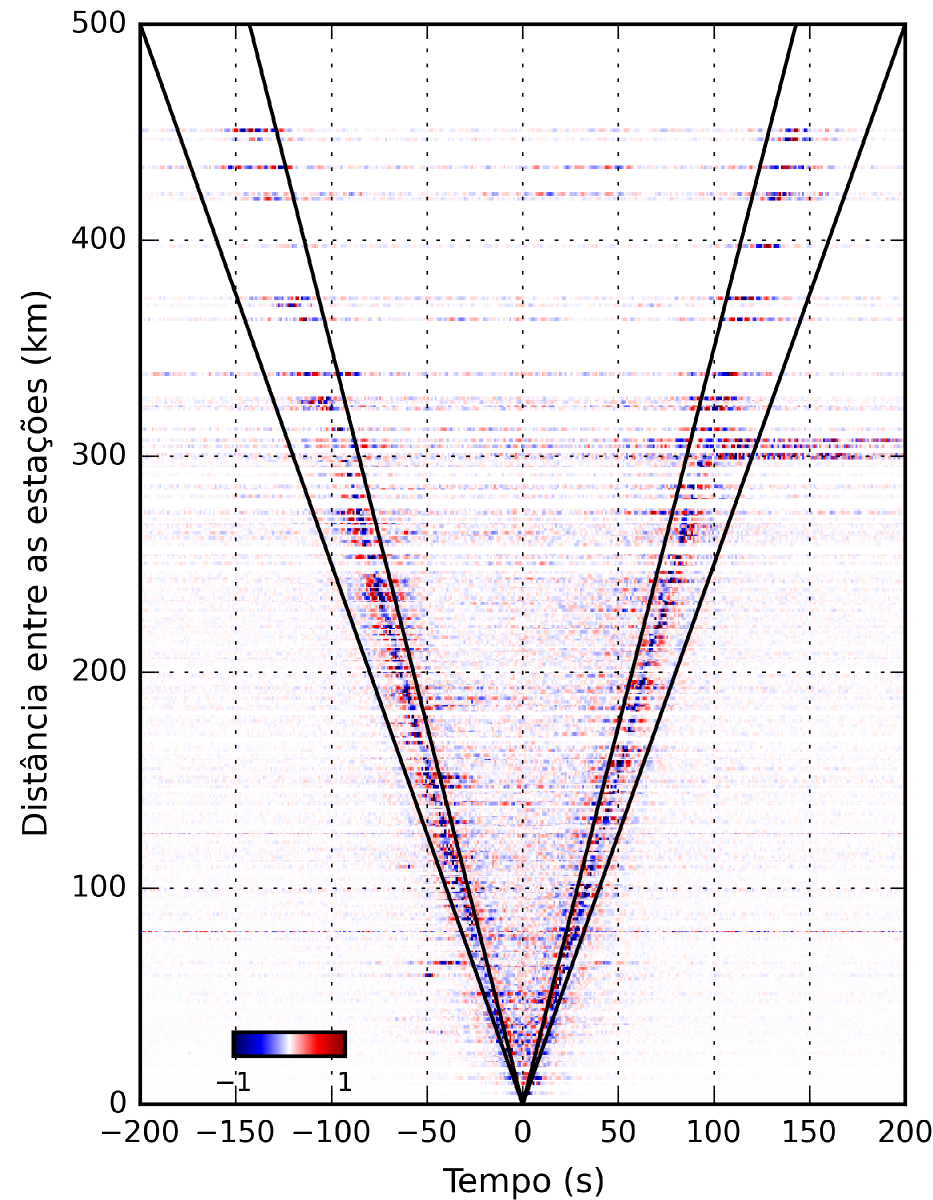
\includegraphics[scale=0.2]{Figs/correlaca_cruzada.png}
\caption[Correlações cruzadas de acordo com a distância entre as estações utilizadas neste trabalho, Tabela \ref{tabelaDATAcorr} (Anexo 3).]{Correlações cruzadas de acordo com a distância entre as estações. Linhas indicam as velocidades de 2.5 e 3.5 $km/s$, faixa de velocidade para as ondas de superfície. Dados foram filtrados por um filtro passa-banda entre 2 e 50 segundos.}
\label{correlacao_cruzada}
\end{figure} 

A correlação cruzada das séries temporais, com tamanho de 1 dia, é feita no domínio do tempo e empilha-se as correlações cruzadas diárias para corresponder a uma longa série temporal. 
O resultado da correlação cruzada são funções do tempo com dois lados, positivo e negativo, com coordenadas em função do tempo, isto é, correlação dos atrasos positivo e negativo, como pode ser visto na Figura \ref{correlacao_cruzada}. O tamanho da série temporal irá depender do grupo de velocidade das ondas e da distância entre as estações.

A parte positiva da correlação cruzada é chamda de sinal "causal" e a parte negativa de "acausal". \cite{bensen_processing_2007} mostra que essas formas de onda representam ondas viajando em direção opostas entre o par de estações, como mostrado na Figura \ref{correlacao_cruzada}. Se as fontes do ruído ambiental são distribuídas homegeneamente em todas as direções, a parte causal e acausal devem ser idênticas. No entanto, assimetrias consideráveis na amplitude e no espectro são observadas, indicando diferenças nas fontes e na distribuição azimutal das mesmas. \cite{bensen_processing_2007} mostra que comprimindo os dois lados do sinal, causal e acausal, em um sinal pode-se aumentar a razão sinal-ruído, o sinal resultante é chamado de sinal simétrico.

\subsection{Medidas da Dispersão}

Após o cálculo e empilhamento das correlações cruzadas diárias, a forma de onda resultante é a função de Green estimada, \cite{campillo_long-range_2003}, \cite{shapiro_emergence_2004} e, principalmente, \cite{wapenaar_retrieving_2004} e \cite{bensen_processing_2007}. Com a função de Green pode-se medir a velocidade de grupo e de fase pela análise frequência-tempo (FTAN), como mostra \cite{levshin_automated_2001}. \cite{bensen_processing_2007} diz que embora FTAN seja aplicada amplamente para fazer medidas das velocidades de grupo, curvas da velcidade de fase também são medidas naturalmente no processo.

\cite{bensen_processing_2007} exemplifica o cálculo da Dispersão das ondas no domínio da frequência por:

\begin{eqnarray}
S_{a}(\omega) = S(\omega)(1 + sgn(\omega))
\end{eqnarray}

onde $sgn(\omega)$ é a função sinal, $S(\omega)$ é a transformada de Fourier da forma de onda $s(t)$, também chamado "sinal analítico".

A transformada inversa é expressa no domínio do temppo por:

\begin{eqnarray}
S_{a}(t) = s(t) + iH(t) = \left | A(t) \right |exp(i\Phi(t))
\end{eqnarray}

onde $H(t)$ é a transformada de Hilbert de $s(t)$. Para construir a função tempo-frequência, o sinal analítico é submetido a um conjunto de filtros Gaussianos passa-banda estreitos com frequências centrais $\omega _{0}$:

\begin{eqnarray}
S_{a}(\omega,\omega _{0}) = S(\omega)(1 + sgn(\omega))G(\omega - \omega _{0})
\\
G(\omega - \omega _{0}) = e^{-\alpha(\frac{\omega - \omega _{0}}{\omega _{0}}^{2})}
\end{eqnarray}

Após a transformação inversa cada função passa-banda é retornada ao domínio do tempo produzindo uma função modulada 2-D, $\left | A(t,\omega _{0}) \right |$, e uma função da fase, $ \Phi(t,\omega _{0}) $. Onde $\alpha$ é o parâmetro que define as resoluções complementares no domínio da frequência e do tempo, \cite{levshin_automated_2001}. O tempo de chegada de grupo, $\tau (\omega _{0})$, como uma função da frequência central do filtro Gaussiano é determinado do pico da função modulada de modo que a velocidade de grupo é $U(\omega _{0})=r/\tau (\omega _{0})$, onde r é a distância entre as estações. \cite{bensen_processing_2007} substitui $\omega _{0}$ pela "frequência instantânea", como mostra \cite{bracewell_fourier_1978}. A frequência instantânea é definida como taxa de variação da fase do sinal analítico num tempo $\tau$. \cite{bensen_processing_2007} declara que esta correção é significativa quando o espectro da forma de onda apresenta picos. Devido ao vazamento espectral as frequências centrais dos filtros de bandas estreitas podem não representar fielmente o conteúdo da frequência de saída dos filtros. \cite{boashash_estimating_1992} explica detalhadamente a utilização da frequência instantânea. Para o processamento utilizou-se a frequência central para a análise tempo/frequência.

A análise frequência-tempo é descrita em duas etapas por \cite{levshin_automated_2001} e \cite{bensen_processing_2007}. A primeira etapa (FTAN bruta), filtros Gaussianos passa-banda estreitos são aplicados na representação analítica da correlação cruzada. Se o período central do filtro é $T$, o tempo em que a amplitude do sinal filtrado chega no máximo corresponde ao tempo de viagem, equivalente a velocidade de grupo $v_{g}$, da onda Rayleigh num período $T$. No entanto, deve-se garantir que a curva de dispersão, $v_{g}(T)$, é uma função suave do período, escapando de saltos causados por máximos espúrios. Isso é feito graças um algoritmo que maxima a soma das amplitudes atravessada pela curva de dispersão, e inclue um termo penalizando descontinuidades na curva.

Essa FTAN bruta é realçada com o uso de um filtro '\textit{phase-matched}', em que o termo de correção $\psi(\omega)$ é aplicado na fase dos sinal analítico no domínio da frequência. $\psi(\omega)$ é avaliado graças à curva de dispersão bruta $v_{g}(T)$ como:

\begin{eqnarray}
\psi(\omega) = \Delta \int_{\omega_{0}}^{\omega} \frac{{d\omega}'}{v_{g}({\omega}')}
\end{eqnarray}

onde $\Delta$ é a distância entre as estações e $\omega = \frac{T}{2\pi}$. Uma curva de dispersão filtrada pode então ser medida repetindo o primeiro passo com o sinal filtrado pelo termo de correção.

A variabilidade estatística das medidas de dispersão é avaliada pelo FTAN e pelas medidas das curvas de dispersão nas correlações cruzadas obtidas dos subconjuntos sazonais trimestralmente (Jan-Fev-Mar, Fev-Mar-Abr, ... , Dec-Jan-Fev). 

\begin{figure}[!ht]
\centering
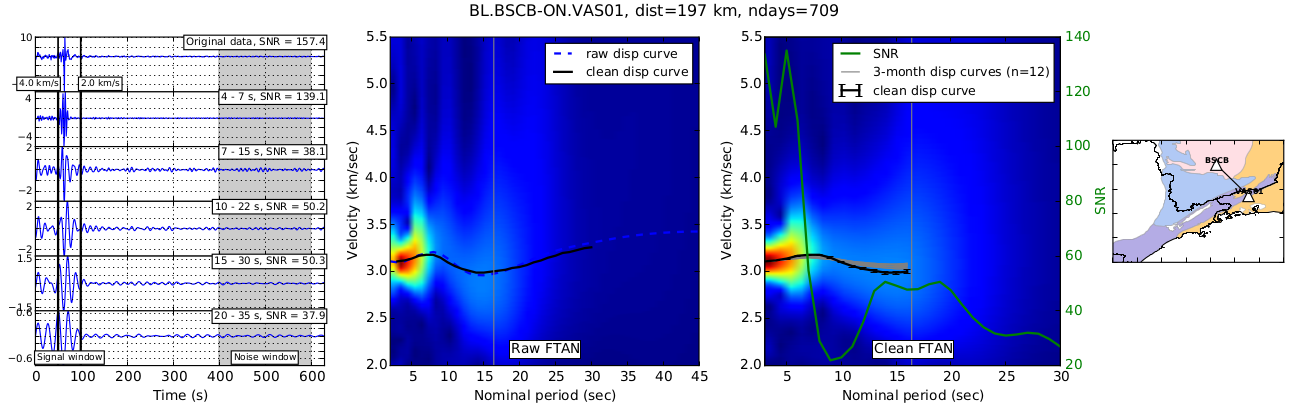
\includegraphics[scale=0.8]{Figs/correlacao_FTAN.png}
\caption[Exemplo de correlação cruzada e análise frequência-tempo (FTAN) no par de estações BL.BSCB-ON.PET01.]{Exemplo de correlação cruzada e análise frequência-tempo (FTAN) no par de estações BL.BSCB-ON.VAS01. (Esquerda) Correlação cruzada original simetrizada e filtrada com passa-banda. (Centro) Amplitude da FTAN bruta e (Direita) filtrada, normalizada por cada valor de período e curvas de dispersão das velocidades de grupo. Os dados da forma de onda foram filtradas entre 2 e 50 segundos. Mapa mostrando a localização do par de estações (estações, províncias tectônicas e divisas estaduais) na parte superior direita.}
\label{correlacao_FTAN}
\end{figure}

A Figura \ref{correlacao_FTAN} ilustra todo o processo para o par de estações BL.BSCB-ON.PET01: cálculo das correlações cruzadas, FTAN bruta, FTAN filtrada, medidas das curvas de dispersão e avaliação da variabilidade sazonal. 

\subsection{Controle de Qualidade das Medidas}

Como a quantidade de caminhos entre as estações é numerosa, o controle de qualidade das correlações cruzadas deverá ser aplicado automaticamente, assim haverá o mínimo de interação humana, logo medidas errôneas serão minimizadas. \cite{bensen_processing_2007} mostra que medidas de dispersão confiáveis devem passar pelo seguinte critério: $\Delta > 3\lambda = 3c\tau$ ou $\tau < \Delta/3c$, sendo $\tau$ o período, $c$ o comprimento de onda, $\Delta$ a distância entre as estações em quilômetros e $\lambda$ o comprimento de onda. Sendo a velocidade de fase máxima ($c$) $\sim 4 km/s$, o período máximo de trabalho é estabelecido por $\tau_{max} = \Delta/12$. \cite{bensen_processing_2007} observa uma degradação das medidas de dispersão em períodos maiores que $\tau_{max}$, como observado na Figura \ref{correlacao_FTAN}. 

Para o controle de qualidade dos dados deve-se identificar e rejeitar medidas ruins. Junto com os critérios estabelecidos por \cite{bensen_processing_2007}, anteriormente, utilizou-se a razão sinal-ruído (SNR), a razão entre o valor máximo absoluto na janela de sinal e o desvio padrão da janela de ruído. Estas janelas são estabelecidas de acordo com a distância entre as estações ($\Delta$). A janela de sinal é demarcada entre os tempos de chegada correspondentes as velocidades de 2.5 e 3.5 $km/s$, mostradas na Figura \ref{correlacao_cruzada}. A janela de ruído é demarcada 200 segundos após a janela de sinal, isso para garantir que seja apenas ruído. O SNR é calculado para cada período aplicando um filtro Gaussiano estreito centrado no período correspondente.

Outro critério estabelecido por \cite{bensen_processing_2007} é avaliar a repetibilidade temporal das medidas de dispersão. As fontes de ruído ambiental mudam sazonalmente e fornecem diferentes condições para as medições. Dadas certas condições de mudança, a repetibilidade da medição é um indicador significativo de confiabilidade. Neste procedimento calculou-se o desvio padrão para um conjunto de velocidades sazonais, estas devem ter SNR maior que 7 e no mínimo 3 dessas velocidades disponíveis. Se não for satisfeito esse critério o desvio padrão é considerado indefinido.

O conjunto de critérios para considerar as medidas de dispersão de boa qualidade para um período $T$ são:

\begin{enumerate}
\item T $\leq$ período de corte, definido no parágrafo anterior;

\item Para velocidades de grupo cujo o desvio padrão é definido: $sigma$ $\leq$ 0.1 km/s e SNR $\geq$ 7;

\item Para velociades de grupo que o desvio padrão é indefinido: SNR $\geq$ 15.
\end{enumerate}

\subsection{Inversão Tomográfica}

A metodologia desenvolvida por  \cite{barmin_fast_2001} foi utilizada para produzir os mapas de velocidade de grupo das ondas Rayleigh. Assume-se que as ondas de superfície seguem os caminhos entre os pares de estações, fazendo com que a inversão seja um problema linear em relação as vagarosidades. Logo num período ($T$) qualquer as pertubações no tempo de viagem entre os pares de estações é dada por:

\begin{equation}
d=Gm
\end{equation} 

O vetor $d$ contém o perturbações no tempo de viagem entre os pares de estações (deduzidos das velocidades de grupo medidas no período $T$), o vetor de parâmetro $m$ consiste da pertubações na vagarosidade ao longo dos nós de um grade regular e a matriz sensibilidade $G$ realiza a integração entre a vagarosidade ao longo do caminho percorrido pelas ondas. As pertubações são relativas ao modelo de referência, definido como a vagarosidade média implícita por todos o tempos de propagação das ondas observados. A vagarosidade modelada é discretizada ao longo de uma grade regular de 0.1º x 0.1º. 

Introduz-se uma função de penalização que é composta por três termos:

\begin{eqnarray}
(Gm-d)^{T}C^{-1}(Gm-d) + \alpha ^{2} \left \| F(m)  \right \| ^{2} + \beta ^{2 } \left \| H(m)  \right \| ^{2}
\end{eqnarray}

O primeiro termo é o desajuste, $C$ é a matriz de covariância dos erros observacionais. $C$ é uma matriz diagonal contendo a variância dos erros nos tempos de viagens observados, deduzidos do desvio padrão das velocidade de grupo, estas velocidades são calculadas previamente. 

O segundo termo da função de penalização é a condição de suavidade espacial, que é dada por:

\begin{eqnarray}
F_{i}(m)=
 \left\{\begin{matrix}
1 \hspace{18mm} if \hspace{3mm} i = j,
\\ 
-S(r_{i},r_{j}) \hspace{3mm} if \hspace{3mm} i \neq j,
\end{matrix}\right.
\end{eqnarray}

\begin{eqnarray}
S(r_{i},r_{j}) \propto exp(- \frac{\left \| r_{i}-r_{j}  \right \|^{2}}{2\sigma ^{2}}) \\
\sum_{j\neq i} S(r_{i},r_{j}) = 1         \forall i 
\end{eqnarray}

com $r_{i}$ a posição do $i$-ésimo nó da grade e $\sigma$ a largura da suavidade espacial.

O terceiro termo penaliza a norma ponderada no modelo, isso faz com que o modelo suavize regiões onde há pouca cobertura de dados:

\begin{eqnarray}
H_{i}(m) = exp(-\lambda \rho _{i})m_{i}
\end{eqnarray}

onde $\rho _{i}$ é o número de caminhos que cruza a célula 0.1º x 0.1º centrada no $i$-ésimo nó da grade. Os parâmetros $\alpha$, $\beta$ ,$\lambda$ e $\sigma$, apresentados na Tabela \ref{tabelaPARAMETROS}, foram ajustados através de otimizações feitas por tentativa e erro.

Para identificar e remover caminhos discrepantes que podem ter passado pelo critério de seleção o procedimento passa-dois foi empregado. Inicialmente um mapa suave de velocidade é produzido através de uma inversão superamortecida. Nesta a maior parte da energia é afetada pela condição de suavidade espacial. Pares que possuem um tempo de viagem residual maior que três vezes o desvio padrão do resíduo, calculado pela diferença entre o tempo de viagem observado e predito,  são descartados. Após isso, uma segunda inversão é feita. O mapa de velocidade gerado por essa segunda inversão é o mapa de velocidade final. A porcentagem de medidas rejeitadas é menos que 2\% em todas as faixas de períodos.

\begin{savenotes}
\begin{table}[!ht]
\begin{center}
\small
\caption{Tabela com os parâmetros utilizados na inversão.}
\begin{tabular}{ l c }
\hline
{\textbf{Parâmetro}} & {\textbf{Valor}}\\
\hline
Grade de Discretização & 0.1º x 0.1º\\
$\alpha$ - Peso do termo de suavidade espacial & 3000,300 \footnote{Primeiro e segundo passo da inversão, respectivamente}
\\
$\sigma$ - Largura da suavidade espacial & 25 km\\
$\beta$ - Peso do termo de penalização da norma & 100\\
$\lambda$ - Nitidez da diminuição da função de ponderação da norma & 0.3\\
\hline
\end{tabular}
\label{tabelaPARAMETROS}
\end{center}
\end{table}
\end{savenotes}

\subsection{Análise da Resolução dos Mapas Tomográficos}

Antes de interpretar os resultados é necessário fazer uma análise da resolução dos dados, necessária para avaliar as limitações dos mapas tomográficos gerados. O processo de inversão descrito nas seções anteriores produz concomitantemente com o resultado uma matriz de resolução para cada ponto na grade. Segundo \cite{barmin_fast_2001} ajusta-se um cone para cada mapa de resolução e reporta o raio deste cone como a resolução espacial característica, isto é interpretado como a distância de separação mínima para duas anomalias para ser resolvido. A resolução não pode ser menor que duas vezes o espaçamento entre os nós. Além disso, cones que possuem os melhores ajustes de altura menores que 10\% da altura máxima são considerados ruído e são automaticamente descartados.  

As limitações dos mapas tomográficos serão avaliadas qualitativamente pelo teste de tabuleiro de damas, \textit{checkerboard}, onde os tempos de viagem observados são substituídos por dados sintéticos gerados de um modelo de anomalias  de velocidade em forma de tabuleiro de damas. O modelo tem alternado anomalias senoidais de $\pm 10\%$ em torno de um valor de velocidade padrão de 3 $km/s$. Em geral, as limitações descritas pelos tabuleiros reconstruídos são consistentes com a resolução espacial estimada.

\section{Resultados}

A análise das pertubações na propagação das ondas de superfície permitem distinguir estruturas crustais intermediárias, que por outros métodos não se tinha resolução. A resolução é controlada pela quantidade de dados e pela distância entre as estações. O foco deste trabalho são as grandes estruturas tectônicas presentes na área, como bacias sedimentares e grandes blocos crustais. A resolução deste trabalho limita-se a valores em profundidade próximos da crosta intermediária.

\subsection{Correlações Cruzadas de Ruído Sísmico Ambiental}

\begin{figure}[!ht]
\centering
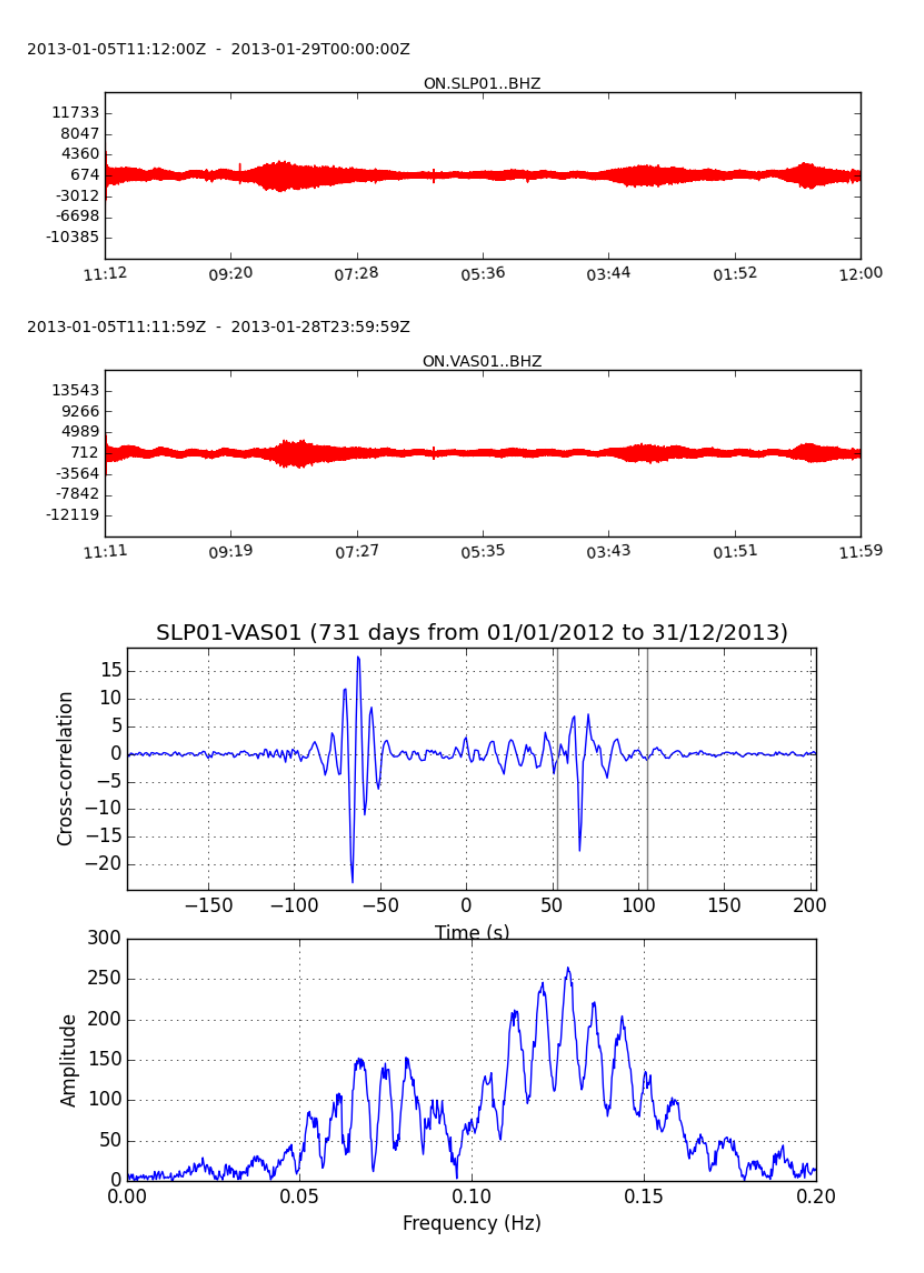
\includegraphics[scale=0.5]{Figs/corr_dado_bruto.png}
\caption[Dados Brutos das estações SLP01 e VAS01 e a correlação dos mesmos.]{Na parte superior da Figura observa-se os dados brutos do mês de Maio das estações SLP01 e VAS01 . Na parte inferior tem-se o empilhamento de 731 dias de correlações cruzadas entre as estações e o espectro deste sinal.}
\label{corr_dado_bruto}
\end{figure}

A parte superior da Figura \ref{corr_dado_bruto} mostra como é o dado após o tratamento, este dado que é processado para gerar as correlações cruzadas. A parte inferior mostra o resultado do empilhamento das correlações cruzadas diárias entre as estações SLP01 e VAS01 em 731 dias, entre os dias 01/01/2012 e 31/12/2013.  A correlação cruzada apresenta uma parte causal (positiva), esta corresponde ao deslocamento de uma onda da estação SLP01 a VAS01, e a anticausal (negativa), que representa a propagação de uma onda entre a estação VAS01 e SLP01. O sinal gerado pela correlação entre as estações SLP01 e VAS01 é assimétrico, Figura \ref{corr_dado_bruto}, assim como a maioria das correlações cruzadas geradas neste trabalho, pode ser observado na Figura \ref{correlacao_cruzada}. No caso da correlação entre SLP01 e VAS01 a maior parte da energia do sinal acumula-se na parte acausal do dado. Isso acontece devido á distribuição das fontes de ruído sísmico ambiental, pois se as fontes fossem azimutalmente bem distribuídas as correlações seriam simétricas, como mostra \cite{stehly_study_2006} em seu trabalho. \cite{stehly_study_2006} mostra a procedência das fontes de rúido sísmico ambiental e explica que as fontes possuem duas bandas espectrais, estas são separadas em primárias (10-20 segundos) e secundárias (5-10 segundos). O ruído sísmico de fundo  de alta frequência, microssismo secundário, é gerado pela interação do oceano com a costa, este tipo de fonte não sofre grandes variações por efeitos sazonais, diferentemente do microssismo primário que exibe uma variação sazonal forte. Portanto a discrepância entre as amplitudes entre as partes causal e acausal da correlação está relacionada com a posição das estações em relação ao oceano. 


\subsection{Análise tempo/frequência}

\begin{figure}[!ht]
\centering
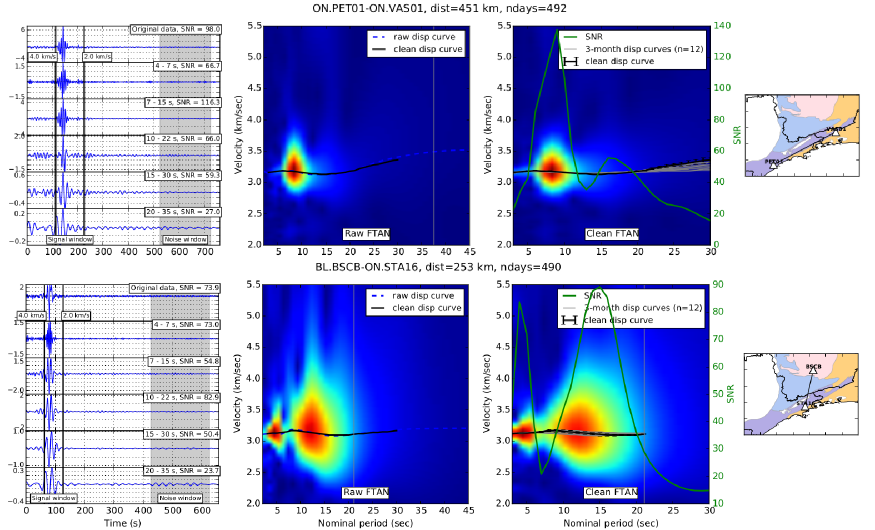
\includegraphics[scale=0.8]{Figs/fonte_FTAN.png}
\caption[Exemplos de correlação cruzada e análise tempo/frequência (FTAN) em dois pares de Estações com configurações espaciais diferentes.]{Exemplos de correlação cruzada e análise frequência tempo (FTAN) em dois pares de Estações com configurações espaciais diferentes. A parte superior mostra um par de estações com uma grande distância mostrando que a maior amplitude do sinal está no período próximo de 10 segundos. Já na parte inferior a amplitude máxima está próxima do período de 4 segundos.}
\label{fonte_FTAN}
\end{figure}

Outro ponto importante sobre as estações em relação a distância do oceano são as amplitude dos gráficos de energa gerados pela análise tempo/frequência. A Figura \ref{fonte_FTAN} e \ref{dist_FTAN} mostram exemplos de quatro pares de estações que possuem configurações distintas e geram alguns resultados interessantes sobre a pespectiva da fonte de ruído. Na Figura \ref{fonte_FTAN} observa-se que os pares em que os trajetos entre as estações estão paralelo à costa a energia contida no sinal concetra-se em volta do período de 7 segundos. Já nos trajetos que estão perpendiculares à costa há uma queda na amplitude do sinal no perído de 7 segundos. Indicando uma forte correspondência com a fonte de ruído sísmico ambiental. A relação entre a distância e a energia mostrado nas análise tempo/frequência pode ser observada na Figura \ref{dist_FTAN}. É notável que quanto maior a distância entre as estações mais informações em profundidade podem ser extraídas das velocidades de grupo. Na figura \ref{dist_FTAN} observa-se essa distribuição de energia bem marcada para ambas distâncias. Em grandes distâncias há uma  espalhamento da energia pelos períodos, porém em curtas distâncias há uma concentração de energia nos pequenos períodos. Nesta dissertação as distâncias entre as estações do projeto SUBSAL varia de $\simeq 20 km$ a $\simeq 50 km$. Portanto, o um grande número de medidas são observadas em curtos períodos com um decaimento linear bem marcado para os períodos mais longos, como pode ser observado na Figura \ref{corr_selecao}. Devido ao acentuado decréscimo do número de medidas para longos períodos, estipulou-se um período máximo para o processamento de 16 segundos, pois tem-se um número de medidas próximo de 100, considerado limite para uma tomografia de qualidade.

\begin{figure}[!ht]
\centering
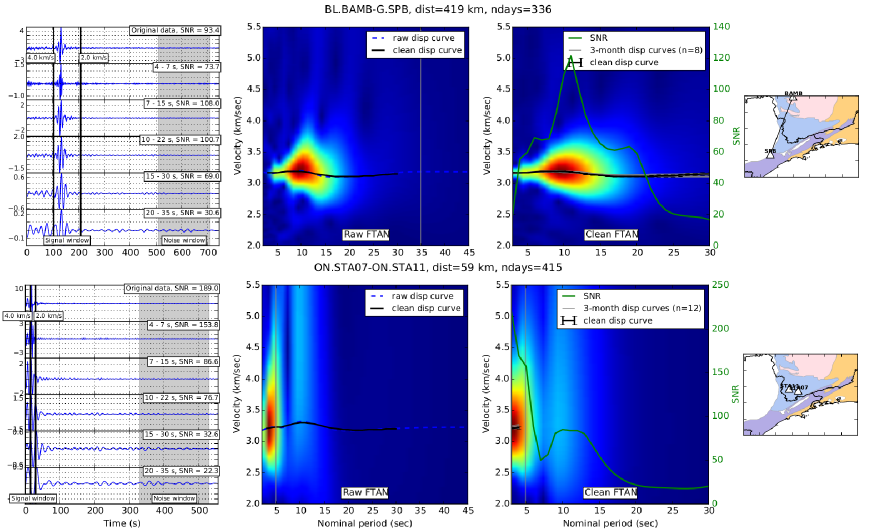
\includegraphics[scale=0.8]{Figs/dist_FTAN.png}
\caption[Exemplos de correlação cruzada e análise tempo/frequência (FTAN) em dois pares de Estações com distâncias diferentes.]{Exemplos de correlação cruzada e análise frequência tempo (FTAN) em dois pares de Estações com distâncias diferentes. A parte superior mostra um par de estações com uma grande distância mostrando que a maior amplitude do sinal está no período próximo de 10 segundos. Já na parte inferior a amplitude máxima está próxima do período de 4 segundos.}
\label{dist_FTAN}
\end{figure}

\begin{figure}[!ht]
\centering
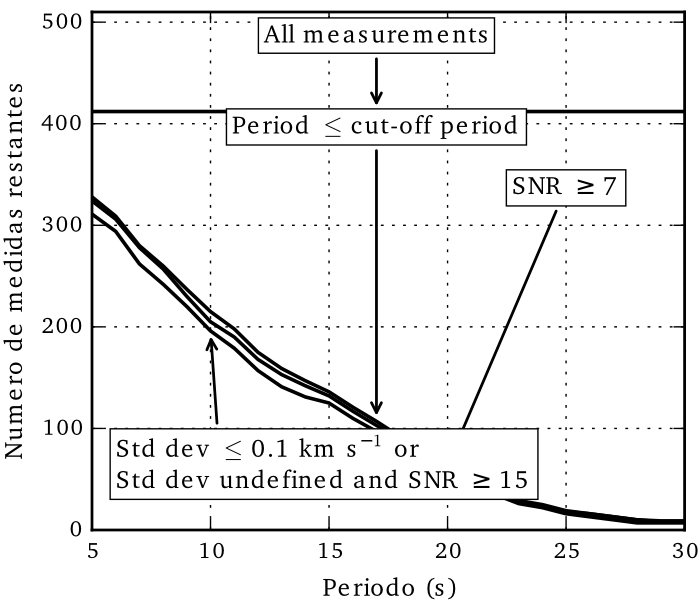
\includegraphics[scale=1]{Figs/corr_selecao.png}
\caption{Efeito do critério de seleção sucessiva na quantidade de medidas de dispersão remanescentes. Os dados de forma de onda foram filtrados entre o passa-banda 2-50 segundos.}
\label{corr_selecao}
\end{figure}

\subsection{Controle de qualidade}

Para analisar qualitativamente as correlações cruzadas utilizadas na tomografia sísmica, comparou-se a razão sinal-ruído em cada período, o resultado pode ser visto na Figura \ref{SNR}. A razão sinal-ruído é calculada pela diferença de amplitude entre a janela de sinal e a janela de ruído. È visível que em curtos períodos as correlações cruzadas possuem um sinal ruído maior, e que há um decrescimento da razão sinal-ruído com o aumento do período. Com isso a resolução em curtos períodos é maior que em longos períodos,

\begin{figure}[!ht]
\centering
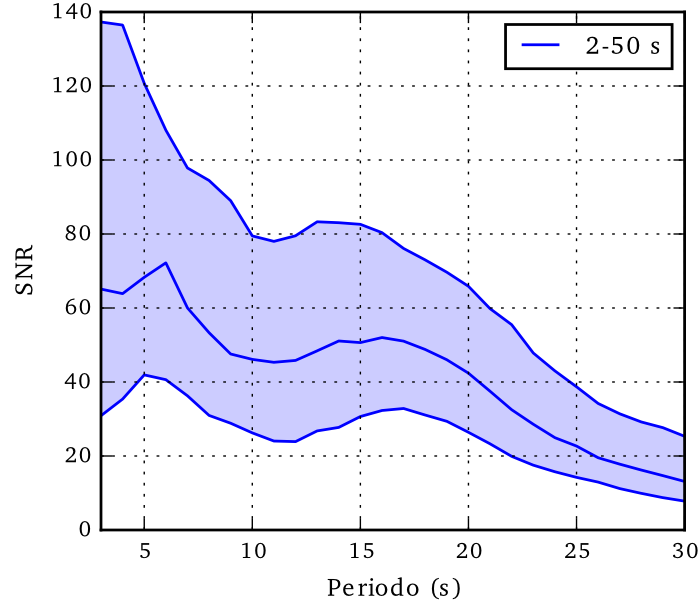
\includegraphics[scale=1]{Figs/SNR.png}
\caption{25\%,50\% e 75\% do  SRN total das correlações cruzadas em função do período. As correlações cruzadas são calculadas com um filtro passa-banda entre 2 e 50 segundos.}
\label{SNR}
\end{figure}

\subsection{Tomografia Sísmica}

A grande quantidade de trabalhos, puramente geológicos ou geológico-geofísicos, produziu uma extensa bibliografia sobre a área, porém não delimitou as estruturas crustais com um certo grau de detalhe. Com a tomografia sísmica tenta-se recuperar essas grandes feições, e para tal testou-se a sensibilidade das velocidades  de grupo das ondas Rayleigh para os seguintes períodos 5, 10 e 16 segundos, Figura \ref{sensibilidade}. Essas sensibilidade foram calculadas para um modelo com essa configuração estrutural: crosta superior de 20 km e crosta inferior de 15 km. Com as sensibilidades calculadas pode-se delimitar a profundidad de atuação de cada período, para este modelo. O período de 5 segundos tem uma sensibilidade de 4 quilômetros, já o modelo de 10 segundos 7 quilômetros e o de 16 segundos de 13 quilômetros, como observado na Figura \ref{sensibilidade}.

\begin{figure}[!ht]
\centering
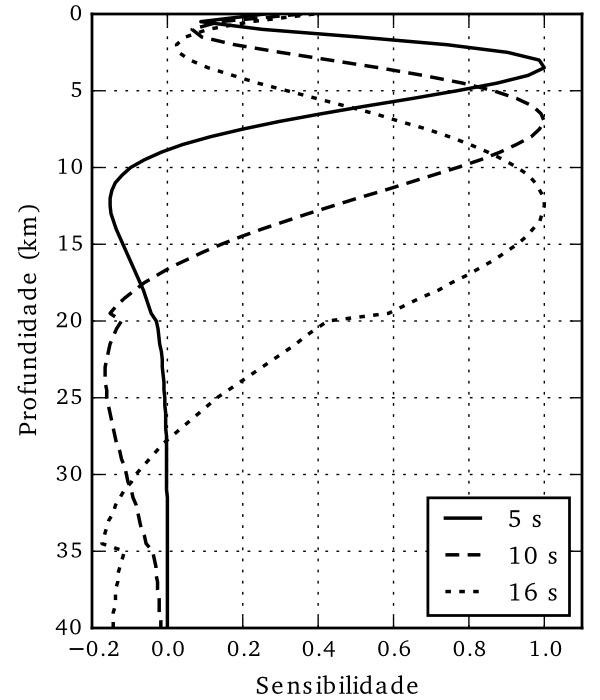
\includegraphics[scale=1]{Figs/sensibilidade.png}
\caption[Sensibilidade das velocidades de grupo das ondas Rayleigh num período selecionado]{Sensibilidade das velocidades de grupo das ondas Rayleigh num período selecionado, normalizada para a unidade. Sensibilidade é definida como a variação na velocidade de grupo causada por uma pequena variação em $V_{s}$ em uma dada profundidade. Essas sensibilidades foram calculadas para um modelo de crosta com uma crosta superior de $20$ km e uma crosta inferior de $15$ km sobre um manto.}
\label{sensibilidade}
\end{figure}

Analisando os mapas de velocidade gerados pela inversão tomográfica, Figura \ref{tomografia}-esquerda, observa-se que as grandes feições estruturais da região foram bem delimitadas nos mapas, como a Bacia do Paraná, Bacia de Taubaté, Faixa Brasília, principalmente no mapa com período de 5 segundos. Os resultados foram descritos tendo como base as unidades tectônicas regionais.

A Bacia do Paraná é a uma grande estrutura regional bem delimitada por todas os mapas tomográficos. O mapa com 5 segundos de período delimita claramente a bacia apresentando uma grande anomalia de baixa velocidade. Porém quanto nos períodos mais longos, 10 e 16, a anomalia de baixa velocidade não é bem delimitada, provavelmente devido a baixa resolução espacial. 

A Bacia de Taubaté também é uma estrutura que possui uma anomalia negativa de velocidade marcante. Mesmo sendo uma bacia pouco profunda é representada nos períodos de 5 e 10 segundos. Já no período de 16 segundos não existe nenhuem indício.

A Faixa Brasília apresenta uma anomalia positiva no período de 5 segundos, porém no período de 10 segundos essa anomalia se torna negativa e no período de 16 segundos volta a ser positiva. Essa mudança de velocidade é um resultado concordante com modelos geofísicos da região, como \cite{sand_franca_crustal_2004}, \cite{flora_solon_ancient_2013} e \cite{Silva_2014}, pois essa mudança estaria relacionada com uma inversão de velocidade devido a Zona de interferência com a Faixa Ribeira. Na parte geológica \cite{trouw_new_2013} mostra a evolução da zona de superposição em que rochas supracrustais são soerguidas gerando o sistema de \textit{Nappes}, mostrado no perfil \ref{perfil_esquematico}, explicando assim essa anomalia de baixa velocidade.

O Cráton do São Franciso possui uma anomalia de velocidade positiva nos mapas de período 5 e 10 segundos, o que era de se esperar de uma área cratônica, porém no mapa de 16 segundos apresenta uma anomalia de velocidade negativa. Tal anomalia encontra-se na Zona de interferência do Cráton com a Faixa Ribeira. \cite{heilbron_serra_2013} mostra que há uma uma imbricação de domínios tectônicos na borda sudeste do Cráton do São Francisco. Nesta amalgamação terrenos metassedimentares Neoproterozóicos, outrora bacias sedimentares, pode ter sidos carreados para grandes profundidades, pois existem sedimentos de arcos magmáticos associados a essa região \citep{heilbron_evolution_2010}, \citep{heilbron_serra_2013} e \citep{trouw_new_2013}. 

A Faixa Ribeira apresenta resultados bem parecidos nos períodos de 5 e 10 segundos, anomalias positivas de velocidade associadas aos arcos Rio Negro, a sudeste, e Socorro, a sudoeste. Uma anomalia negativa de velocidade associada a Bacia de Taubaté e a região costeira próxima ao litoral sul de São Paulo, podendo ter influência de bacias sedimentares costeiras. Uma característica interessante é a anomalia de baixa velocidade na região sudoeste da Faixa Brasília no mapa de 16 segundos, porém não foi encontrado na literatura algo que faça referência a essa anomalia de baixa velocidade. Essas anomalias negativas devem ser tratadas com cuidado, pois estão localizadas nos limites dos mapas tomográficos e assosciadas somente a uma estação. 

\begin{figure}[!ht]
\centering
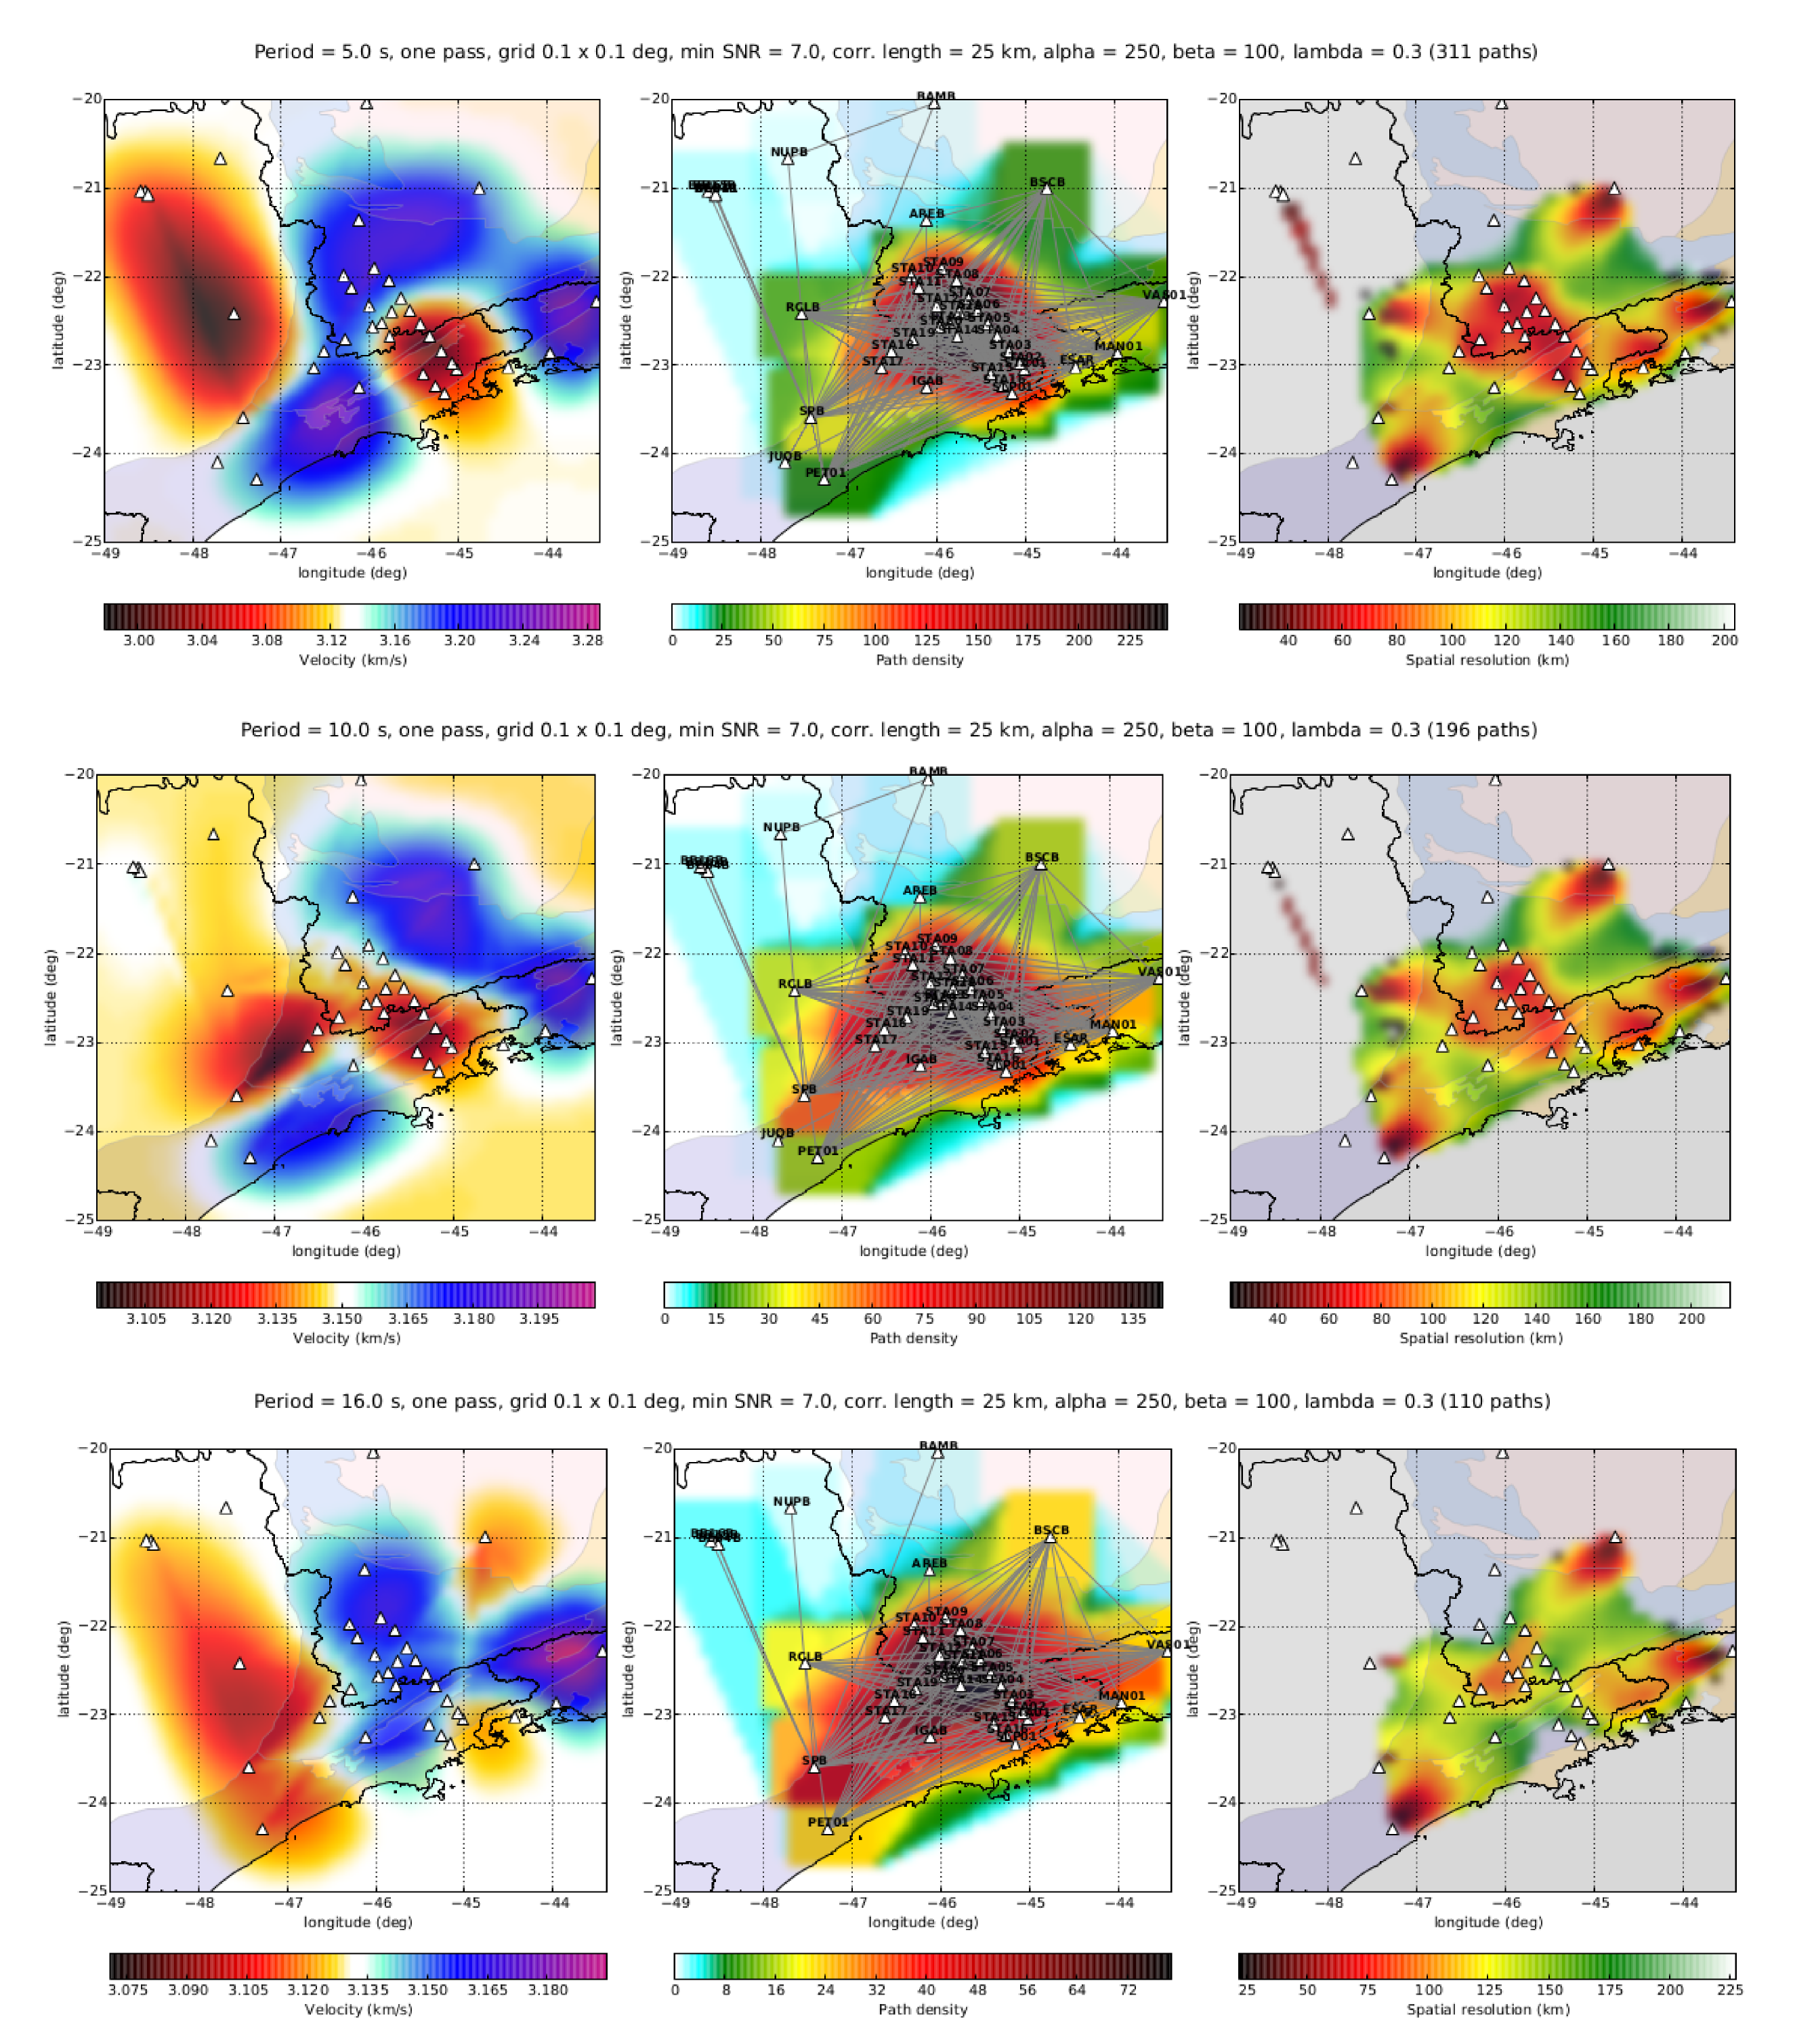
\includegraphics[scale=0.45]{Figs/mapa_tomografia.png}
\caption[Mosaico contendo as pertubações nas velocidades de grupo, trajetórias entre as estações e a resolução espacial.]{Esquerda: Pertubações nas velocidades de grupo nas ondas Rayleigh relativas a velocidade média sobre o mapa no períodos de 5, 10 e 16 segundos. Centro: Trajetórias entre as estações válidas para a inversão tomográfica. Direita: Resolução espacial definida como o raio do cone que melhor ajusta o mapa de resolução em cada ponto. Ao fundo encontra-se o mapa geológico da regional.}
\label{tomografia}
\end{figure}

As colunas central e direita da Figura \ref{tomografia} mostram a densidade de trajetórias e a resolução espacial para a tomografia sísmica. Os resultados tiveram como base a resolução espacial da tomografia. Nota-se claramente que com o aumento do período há uma diminuição da resolução espacial devido a redução do número de caminhos. A região que possui a melhor resolução espacial é a região em que se localiza a rede SUBSAL.

\pagebreak
